\section{Controlled signed-shape identity and near-geometry safeguards}
These results are a separate controlled study, rather than a replacement selected from the outer-test scores. Labels, energy grid, physical top-two layers and inherited outer query records are unchanged. All scalers, feature selection and thresholds use training partitions. Identity can use a documented normalized signed difference without absolute per-Cu calibration; absolute coverage remains a separately calibrated target. Null signals are not converted into unit-norm apparent signals.

Element-aware atom matching uses in-plane minimum-image distances and no vacuum wrapping. Same-composition, same-connectivity records with root-mean-square displacement at most0.02\,\AA\ and maximum atom displacement at most0.2\,\AA\ are assigned to conservative near-geometry groups. This geometry-only definition was fixed before the guarded fits. Six pairs meet it: three also meet the stricter maximum0.05\,\AA\ rule. Very close H-covered aliases and two CHO-containing mixtures cross the inherited folds; the directory coverage label alone does not define their observed loading. These are related geometry groups, not independently verified clean-parent families.

The130 identity records span124 conservative groups:118 Cu--Au records span112 groups and12 Cu(100) records span12 groups. The original99-query control spans96 groups, so the19 added records contribute16 groups. CHO support is nine positive records in eight groups, including two pure records; H support is30 positive records in27 groups. COCHO still has a single positive. Atom/molecule counts, contact definitions and all labels are held fixed.

To preserve the requested outer query folds while preventing related states from entering training, every group represented among the outer queries is removed from that outer training partition. Training uses one canonical available member per remaining group, preferring an older audited record when available. Inner validation obeys the same protection, with inherited old-training assignments preserved. Every physical layer and repeated view remains attached to its geometry group. Equal-group metrics give one total weight to related query records; grouped bootstrap intervals resample these groups together across fixed seed predictions.

\begin{table}[!htbp]\centering\scriptsize
\caption{Fixed Combined representation, threshold0.5, logistic $C=1$ or independent balanced64-tree leaf1 anchor. Values are micro F1 with equal near-geometry-group weights. No feature or estimator is chosen using these outer scores.}
\begin{tabular}{lrrrr}\toprule
Input & Cu--Au logistic & Cu--Au trees & Joint logistic & Joint trees\\\midrule
Native-normalized raw & 0.6266 & 0.7123 & 0.5611 & 0.7167\\
Corrected-normalized raw & 0.6319 & 0.7045 & 0.5457 & 0.7155\\
Common-scale raw & 0.6344 & 0.7153 & 0.5671 & 0.6989\\
Relative signed difference & 0.6344 & 0.7153 & 0.5788 & 0.6940\\
Guarded signed shape & 0.6647 & 0.7500 & 0.6500 & 0.7602\\
\bottomrule\end{tabular}\end{table}

The signed-shape transform is $d_s(E)=d(E)/\sqrt{N^{-1}\sum_j d(E_j)^2}$ only above a training-defined floor. Below it, the signal remains zero and inference abstains. An already unit-normalized experimental input must provide pre-normalization signal-to-noise evidence; no absolute raw pair is required. The floor is a heuristic, not an experimentally validated detection limit. Difference normalization is identity-oriented and is not used to infer absolute coverage.

In joint training, signed shape improves fixed-logistic micro F1 by0.0712 with a conditional group-bootstrap95\% interval[0.0323,0.1094], and the tree control by0.0662[0.0231,0.1171]. On Cu--Au alone the respective intervals include zero. Centered regularized logistic models give identical Cu--Au common-scale-raw and difference predictions: subtracting one fixed reference offset cannot add information after training centering. Differences between source correction, normalization and subtraction must therefore not be attributed to a single mechanism.

\begin{table}[!htbp]\centering\scriptsize
\caption{Differential Combined/tree training-size control, averaged over all three fixed seeds on identical old99 query records (96 near-geometry groups). Intervals condition on saved predictions; seed/refit variation is separately recorded.}
\begin{tabular}{lrrr}\toprule
Threshold rule & Old training & Expanded training & Paired difference95\% interval\\\midrule
fixed0p5 & 0.7130 & 0.7252 & [-0.0234, 0.0495]\\
transferred & 0.7191 & 0.7295 & [-0.0190, 0.0425]\\
common & 0.7191 & 0.7311 & [-0.0157, 0.0415]\\
\bottomrule\end{tabular}\end{table}

The grouping cutoff matters. With the stricter maximum0.05\,\AA\ rule, only three pairs are grouped; the fixed0.5 training-size mean rises from0.7007 to0.7431, with conditional interval[0.0061,0.0815] for the difference. The conservative six-pair grouping weakens this conclusion and its intervals include no improvement. Neither cutoff was selected to maximize test performance. Historical unguarded predictions remain an explicit earlier scope, not independent evidence.

Thirty additional pair-first robustness models compare normalized raw, relative difference and signed shape on the same supported interior8975--9028\,eV window. Shared and residual registration errors, shared-reference plus independent noise, common acquisition gain, residual sample gain and additional Gaussian broadening are separate scenarios. Common acquisition gain changes both members and their shared divisor and cancels. Residual gain or reference-only shifts can severely alter the weak difference. Training-only paired augmentation trades clean-spectrum accuracy against some stressed cases; it does not establish measured experimental accuracy. One reference family per domain prevents new-parent validation, and the small Cu(100) support cannot establish facet transfer. Full single/mixed, per-label, false-positive, abstention, domain-held-out and uncertainty tables accompany this study.

\begin{figure}[!htbp]\centering
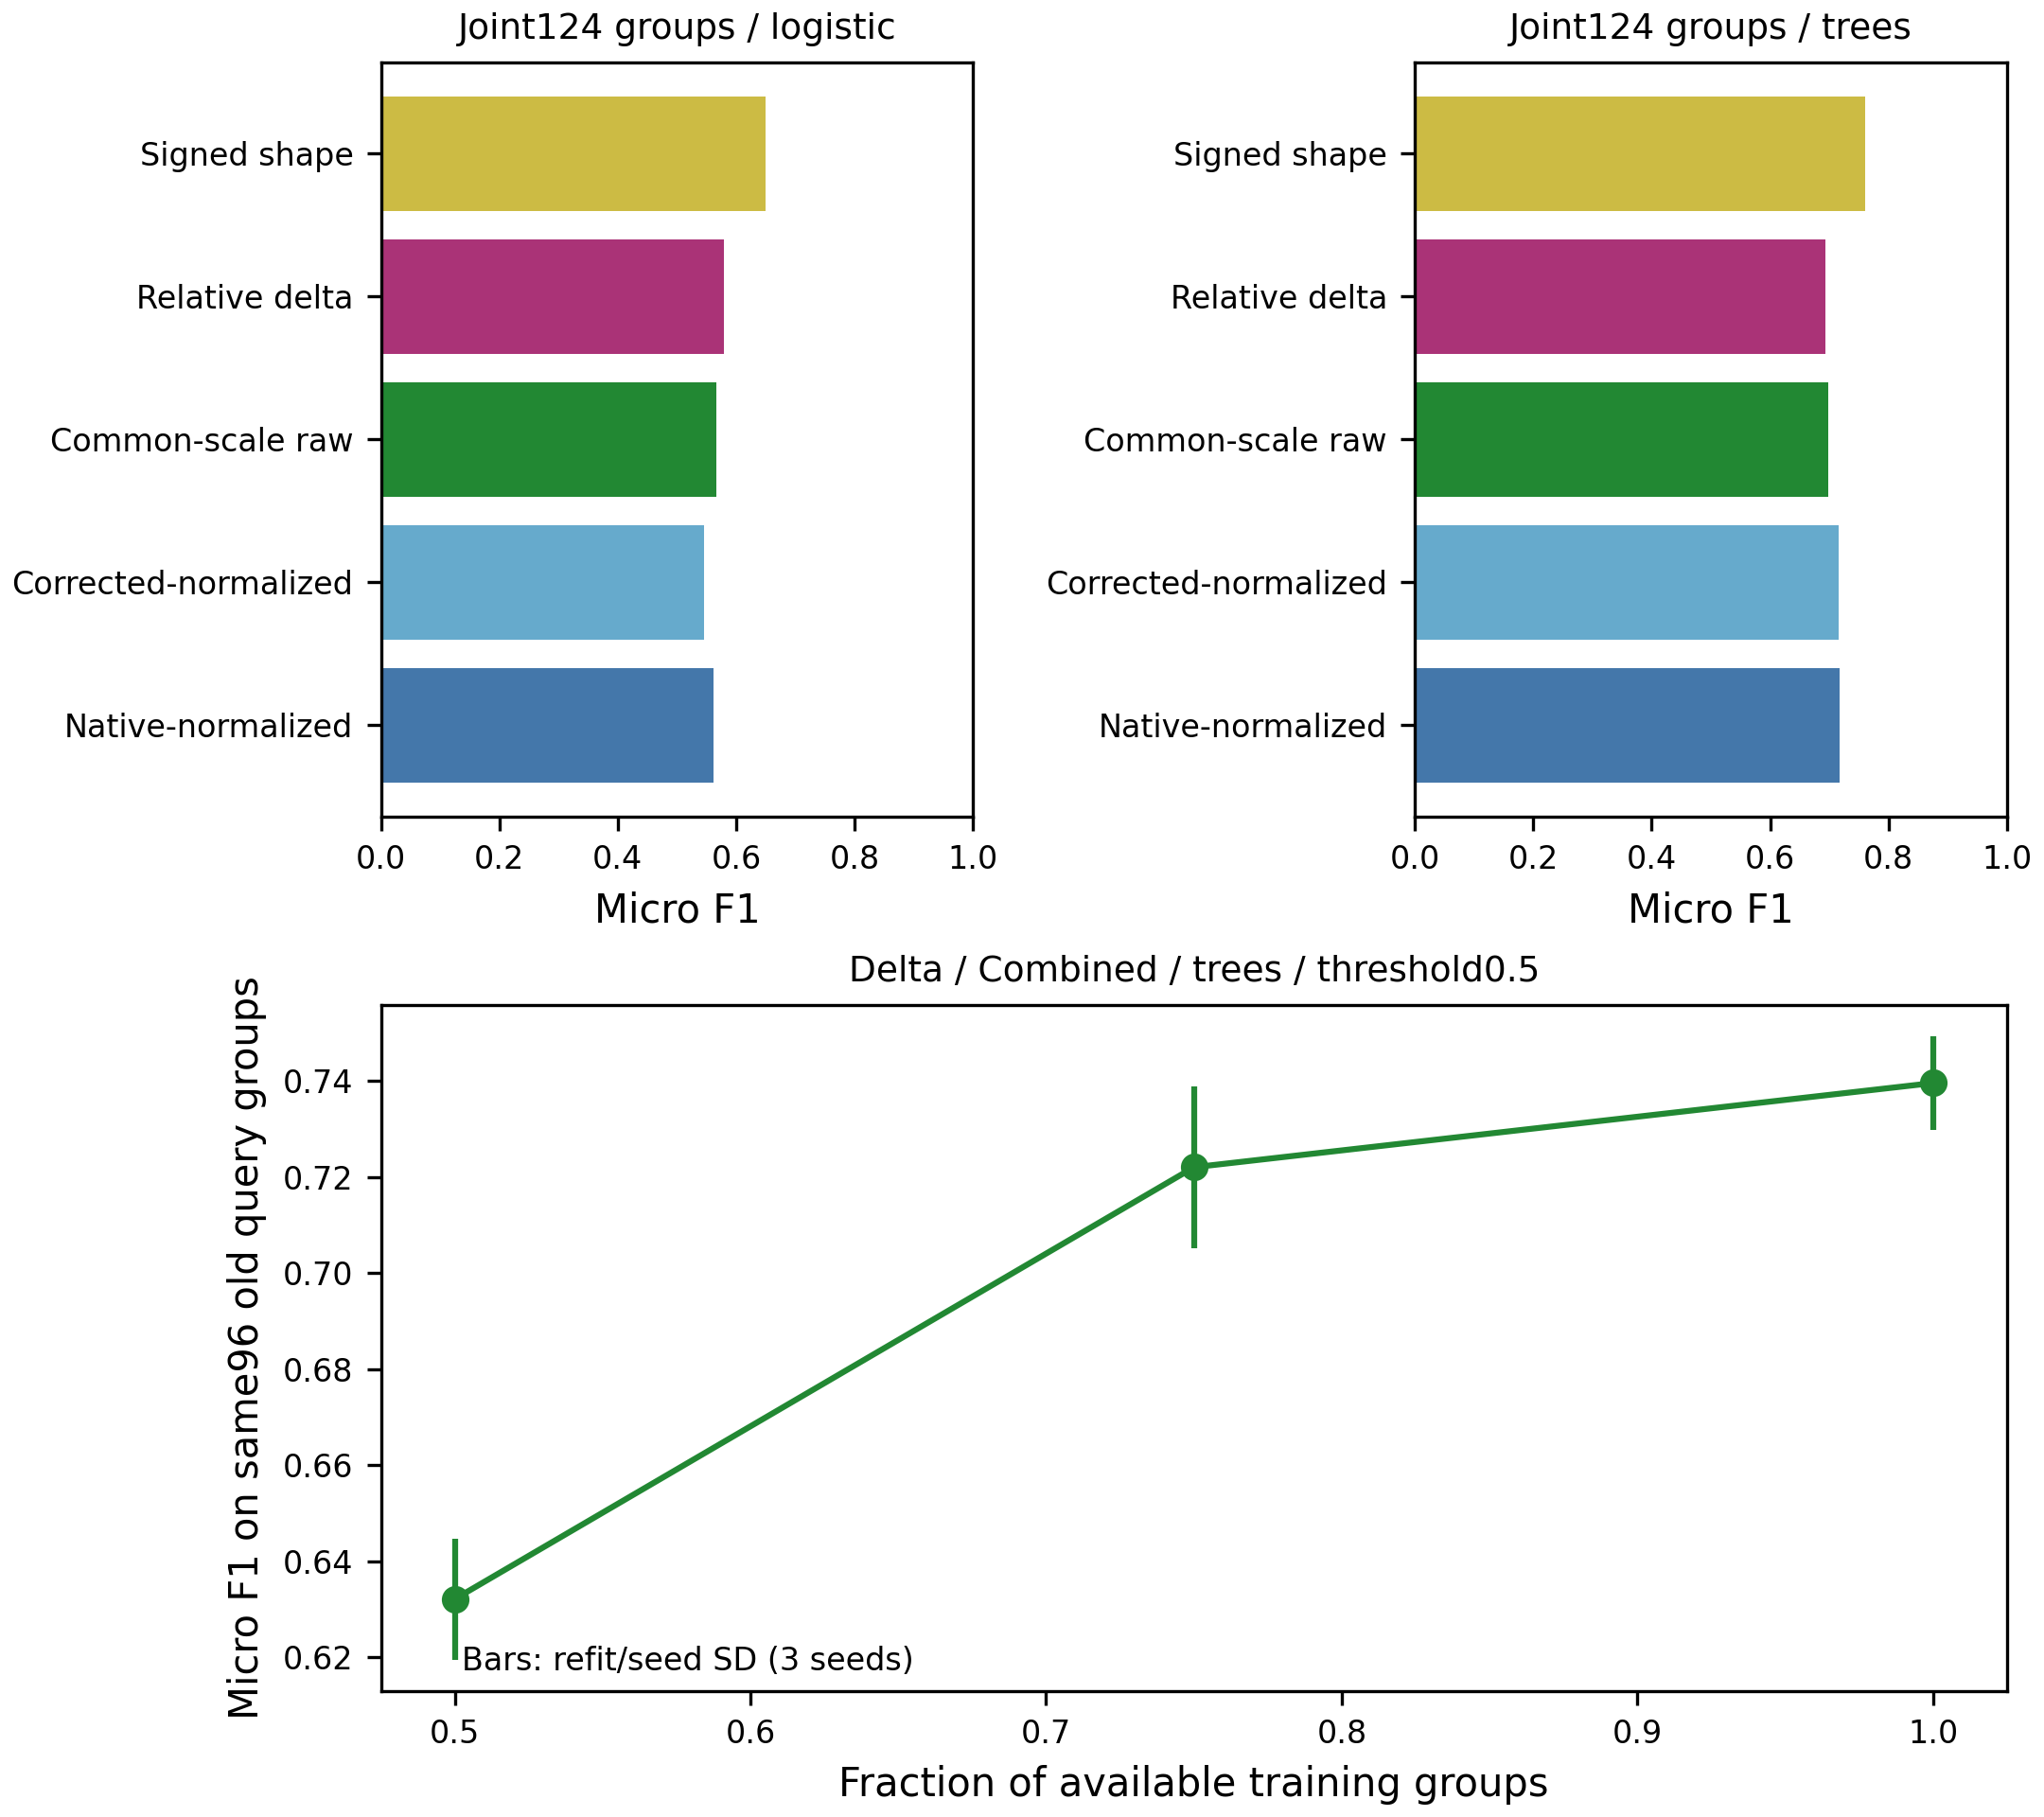
\includegraphics[width=\textwidth]{figures/SI_controlled_identity.png}
\caption{Guarded fixed-recipe controls and genuinely group-sampled learning curves. All panels give equal near-geometry-group weights. Joint-training bar panels evaluate124 query groups. Learning subsets are sampled from canonical training groups after excluding every query-related group, keeping the same96 original query groups. All three seeds are shown; error bars are seed/refit standard deviations, not bootstrap intervals or independent confirmation.}
\end{figure}
